\chapter{Diseño e implementación} % Main chapter title

A continuación se describirá la solución implementada en el trabajo. Se mostrará la arquitectura utilizada, se comentará como fue el pre procesamiento y análisis de datos. También se analizarán los modelos de inteligencia artificial implementados, su arquitectura y particularidades. Por último se analizará el software integrador implementado.

\label{Chapter3} % Change X to a consecutive number; for referencing this chapter elsewhere, use \ref{ChapterX}

\definecolor{mygreen}{rgb}{0,0.6,0}
\definecolor{mygray}{rgb}{0.5,0.5,0.5}
\definecolor{mymauve}{rgb}{0.58,0,0.82}

%%%%%%%%%%%%%%%%%%%%%%%%%%%%%%%%%%%%%%%%%%%%%%%%%%%%%%%%%%%%%%%%%%%%%%%%%%%%%
% parámetros para configurar el formato del código en los entornos lstlisting
%%%%%%%%%%%%%%%%%%%%%%%%%%%%%%%%%%%%%%%%%%%%%%%%%%%%%%%%%%%%%%%%%%%%%%%%%%%%%
\lstset{ %
  backgroundcolor=\color{white},   % choose the background color; you must add \usepackage{color} or \usepackage{xcolor}
  basicstyle=\footnotesize,        % the size of the fonts that are used for the code
  breakatwhitespace=false,         % sets if automatic breaks should only happen at whitespace
  breaklines=true,                 % sets automatic line breaking
  captionpos=b,                    % sets the caption-position to bottom
  commentstyle=\color{mygreen},    % comment style
  deletekeywords={...},            % if you want to delete keywords from the given language
  %escapeinside={\%*}{*)},          % if you want to add LaTeX within your code
  %extendedchars=true,              % lets you use non-ASCII characters; for 8-bits encodings only, does not work with UTF-8
  %frame=single,	                % adds a frame around the code
  keepspaces=true,                 % keeps spaces in text, useful for keeping indentation of code (possibly needs columns=flexible)
  keywordstyle=\color{blue},       % keyword style
  language=[ANSI]C,                % the language of the code
  %otherkeywords={*,...},           % if you want to add more keywords to the set
  numbers=left,                    % where to put the line-numbers; possible values are (none, left, right)
  numbersep=5pt,                   % how far the line-numbers are from the code
  numberstyle=\tiny\color{mygray}, % the style that is used for the line-numbers
  rulecolor=\color{black},         % if not set, the frame-color may be changed on line-breaks within not-black text (e.g. comments (green here))
  showspaces=false,                % show spaces everywhere adding particular underscores; it overrides 'showstringspaces'
  showstringspaces=false,          % underline spaces within strings only
  showtabs=false,                  % show tabs within strings adding particular underscores
  stepnumber=1,                    % the step between two line-numbers. If it's 1, each line will be numbered
  stringstyle=\color{mymauve},     % string literal style
  tabsize=2,	                   % sets default tabsize to 2 spaces
  title=\lstname,                  % show the filename of files included with \lstinputlisting; also try caption instead of title
  morecomment=[s]{/*}{*/}
}


%----------------------------------------------------------------------------------------
%	SECTION 1
%----------------------------------------------------------------------------------------
\section{Arquitectura general del sistema}
 Sea $x$ el vector de datos de entrada, el objetivo es consturir un modelo cuya salida $y$ sea la temperatura del agua que debe circular por el equipo para que la temperatura del paciente se aproxime a la objetivo. Se definen tres valores protagonistas. Por un lado, el vector de entrada $x$, por otro lado la salida del modelo $y$, y por otro lado la temperatura a la que se lleva al paciente $y'$ si la temperatura del agua en el equipo es $y$.
Se define la función \ref{eq:f_x} como la relación entre $x$ y la temperatura del agua.

\begin{equation}
	\label{eq:f_x}
	y = f(x)
\end{equation}

La función \ref{eq:gx} es la relación entre $x'$ y la temperatura del paciente, siendo $x'$ el vector $x$ incluyendo como temperatura del agua a $y = f(x)$.

\begin{equation}
	\label{eq:gx}
	y' = g(x')
\end{equation}

Se define a la temperatura a la que se lleva al paciente como la composición de las funciones \ref{eq:f_x} y \ref{eq:gx} en la función \ref{eq:h_x}.

\begin{equation}
	\label{eq:h_x}
	y' = g(x \circ fx))
\end{equation}

A partir de estas funciones se ve que se deben representar dos relaciones. En primer lugar, dado un vector de datos de entrada $x$, cómo influye en la temperatura que tendrá el paciente en el siguiente periodo de tiempo, y en segundo lugar, dado un vector de datos de entrada $x$ cuál es la temperatura óptima del agua. Las dos relaciones son necesarias para el trabajo y ambas deben ser resueltas a partir de los datos. Para resolver estas relaciones se implementaron dos modelos de inteligencia artificial.

La arquitectura de los modelos implementados para representar estas funciones se muestra en la figura \ref{fig:architecture}. 

\vspace{1cm}

\begin{figure}[htbp]
	\centering
	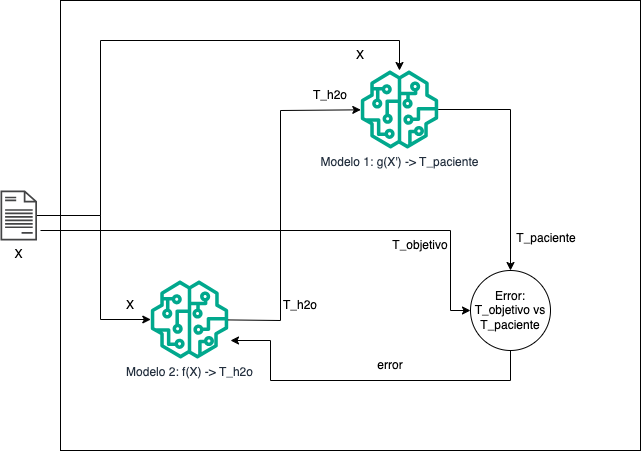
\includegraphics[width=1\textwidth]{./Figures/arquitectura_v2.png}
	\caption{Arquitectura de modelos del trabajo.}
	\label{fig:architecture}
\end{figure}

El modelo 1 implementa a la función \ref{eq:gx}. Fue entrenado en primera instancia a partir los datos del conjunto de datos recibido por el cliente. 
El modelo 2 implementa a la función \ref{eq:f_x}. Para entrenar este modelo la función de error no fue estándar. No existe, a priori, un vector $y$ con los valores certeros a los que el modelo 2 debe definir la temperatura del agua. Para entrenar al modelo 2 se debió utilizar al modelo 1, como se muestra en el círculo que representa a la función del error. El error se define como la diferencia entre la temperatura a la que se lleva al paciente con la salida del modelo y la objetivo. 
Se debe tener en cuenta que para definir a que temperatura se lleva al paciente dado un conjunto de datos se utiliza un modelo, que se entrenó a partir de los datos, y tiene un error en sus predicciones. 
Para el entrenamiento del modelo 2 no se deben modificar los pesos del modelo 1. Este último ya fue entrenado y debe utilizarse como caja negra. 
Se puede resolver este problema con un sólo modelo, cuyas últimas capas se entrenen en una etapa y sus primeras etapas, después. Pero este enfoque es mas complejo de implementar y ofrece menor claridad conceptual, por lo que se optó por la solución planteada.


\section{Análisis de los datos}
La empresa envío datos del tratamiento de casi 100 pacientes. Los datos estaban representados en tres formatos diferentes correspondientes a versiones del software del equipo, y en archivos de extensión .txt y .xlsx.
El equipo realiza una medición cada 15 minutos. Por esto cada tratamiento esta representado con dos secciones. La primera con información del paciente. De esta sección se consideraron el peso y la edad, ignorando cualquier dato identificatorio para resguardar la privacidad del paciente. La segunda consta de un conjunto con todas las mediciones realizadas por el equipo cada 15 minutos durante todo el tratamiento. 

Los datos considerados son los siguientes:
\begin{itemize}
	\item EDAD, en días.
	\item PESO, en gramos.
	\item FECHA INICIO, inicio del tratamiento.
	\item REG: Número de Registro.
	\item T\_SP: Temperatura objetivo.
	\item T\_H2O: Temperatura del agua que absorbe el calor del paciente.
	\item T\_PAC: Temperatura del paciente.
	\item MODO DE USO: Indica el modo de uso configurado.
	\item RAMPA\_HAB: Modo rampa habilitada, esto es influir en la temperatura del paciente para llevarla hacia el objetivo o hacia la normal, o deshabilitada, que consiste en mantener la temperatura estable.
	\item RAMPA\_SET: Indica la tasa de recalentamiento configurada para la función de rampa en °C / h.
	\item FECHA, de la medición.
\end{itemize}

La distribución de las temperaturas de los pacientes se muestran en la figura \ref{fig:pac}. La de las objetivo, en la figura \ref{fig:sp}, y la del peso de los pacientes en la imagen \ref{fig:peso}.
Se ven algunos valores extremos, como temperaturas de pacientes cercanas a los 0 ºC. Se verá en la siguiente sección el tratamiento que se da a estas anomalías. 

\begin{figure}[htbp]
\centering
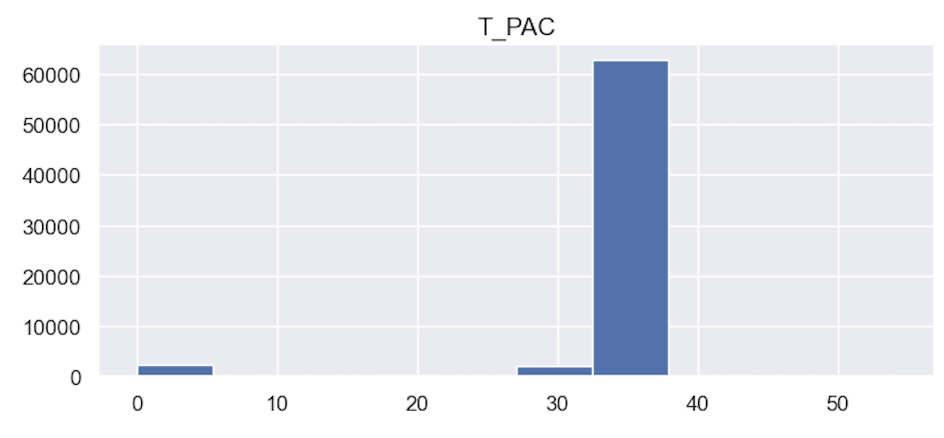
\includegraphics[width=0.5\textwidth]{./Figures/dist_t_pac.png}
\caption{Distribución de temperaturas de los pacientes.}
\label{fig:pac}
\end{figure}

\begin{figure}[htbp]
	\centering
	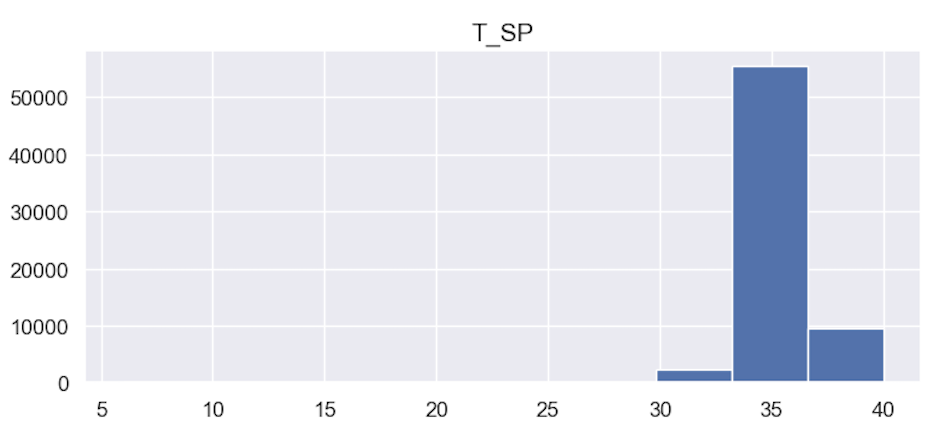
\includegraphics[width=0.5\textwidth]{./Figures/dist_sp.png}
	\caption{Distribución de temperaturas objetivo.}
	\label{fig:sp}
\end{figure}


\begin{figure}[htbp]
	\centering
	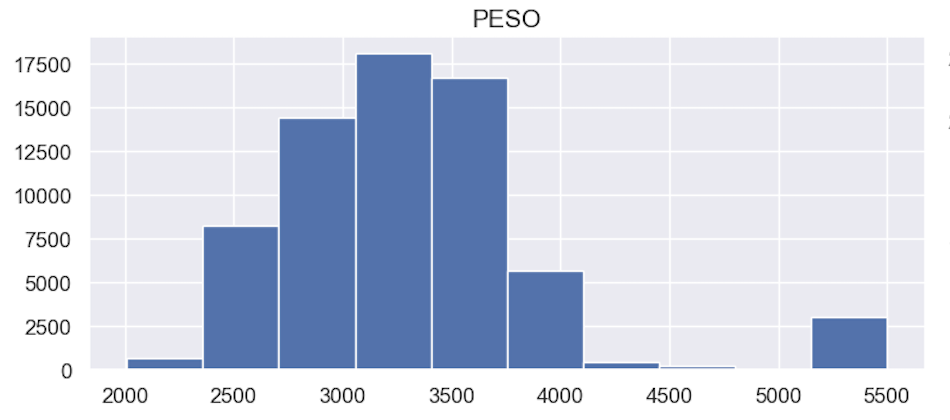
\includegraphics[width=0.9\textwidth]{./Figures/dist_peso.png}
	\caption{Distribución de pesos de los pacientes.}
	\label{fig:peso}
\end{figure}

En la figura \ref{fig:corr} se muestra la correlación entre las variables de los datos recibidos.
\begin{figure}[htbp]
	\centering
	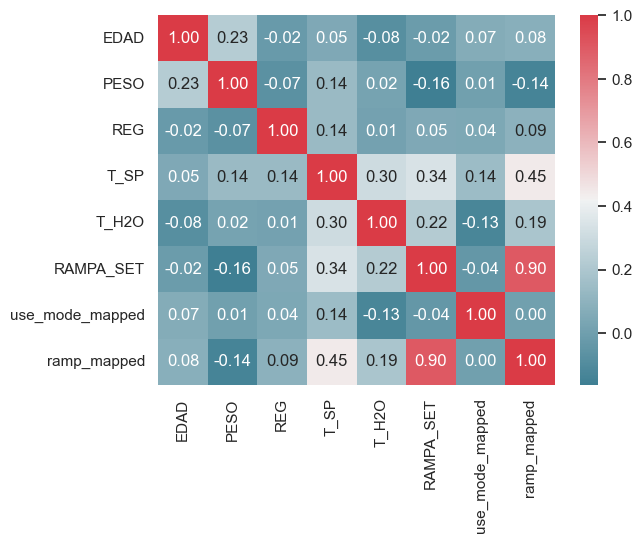
\includegraphics[width=0.9\textwidth]{./Figures/correlation.png}
	\caption{Correlación entre las variables.}
	\label{fig:corr}
\end{figure}

\section{Preprocesamiento de datos}
